% !TEX encoding = UTF-8 Unicode
% !TEX program = pdflatex
% !TEX spellcheck = en_US


% In order to correctly compile this document,
% execute the following commands:
% 1. pdflatex
% 2. pdflatex
% 3. pdflatex



\documentclass[amsthm,ebook]{saparticle}

% IF YOU USE PDFLATEX
\usepackage[utf8x]{inputenc}
% if you write in english and in greek
\usepackage{ucs}
\usepackage[greek,english]{babel}
\languageattribute{greek}{polutoniko}

\usepackage{graphicx}
\newlength{\xbreite}
\settowidth{\xbreite}{x}
\newcommand*{\chirho}{\scalebox{2}[1.2]{x}\hspace*{-1.25\xbreite}\scalebox{.5}[1.5]{\bfseries P}}

% IF YOU USE XELATEX
%\usepackage{polyglossia}
% if you write in italian
%\setmainlanguage{italian}
% If you want put some ancient greek:
%\setotherlanguage[variant=polytonic]{greek}
%\newfontfamily{\greekfont}[Ligatures=TeX]{Palatino Linotype}

% dummy text (remove in a normal thesis)
% remove if not necessary
\usepackage{siunitx}
%Natbib for bibliography management
\usepackage[authoryear]{natbib}
% custom commands
\newcommand{\bs}{\textbackslash}

%%%%%%%%
%TITLE:%
%%%%%%%%
\title{Towards the Publication of ICI Siracusa: General Data and Previews.}
\author[unica]{Mariarita Sgarlata\corref{first}}
\address[unica]{Department of Humanities - University of Catania} 
\cortext[first]{Corresponding author. Email: m.sgarlata@unict.it}
\begin{document}
\maketitle
\begin{abstract}
This paper refers to the general track ``Epigraphic edition on paper and on line''. Some researchers who has been working on the editing of the \emph{Inscriptiones Christianae Italiae}, published from the University of Bari, contributed also to the EDR project, that collect on line the epigraphic documents of Roman Christian Period. I propose a preview of the work currently in progress, with a specific reference to the inscriptions that provide us the chronological and topographic data to study the cemetery as well as formularies linked to the society structure and to the identity-making characteristics.
\end{abstract}
\keywords{Sicily, Syracuse, Epigraphy, Topography, Society, Onomastic and Identity}

\section{General Data about Epigraphs}

%\begin{figure}[hbp]
%\centering
 %\includegraphics[width=\columnwidth]{MISSING IMAGE!}
%\caption{The main gallery (so called \emph{decumanus}) of Catacombs of San Giovanni}
%\label{fig:1}
%\end{figure}

\noindent We are far from a complete and thorough research about palaeochristian epigraphs in Sicily. This catalogue represents the first step of a systematic study focused on the inscriptions discovered in the christian cemeteries of Siracusa.

\begin{figure}[hbp]
\centering
 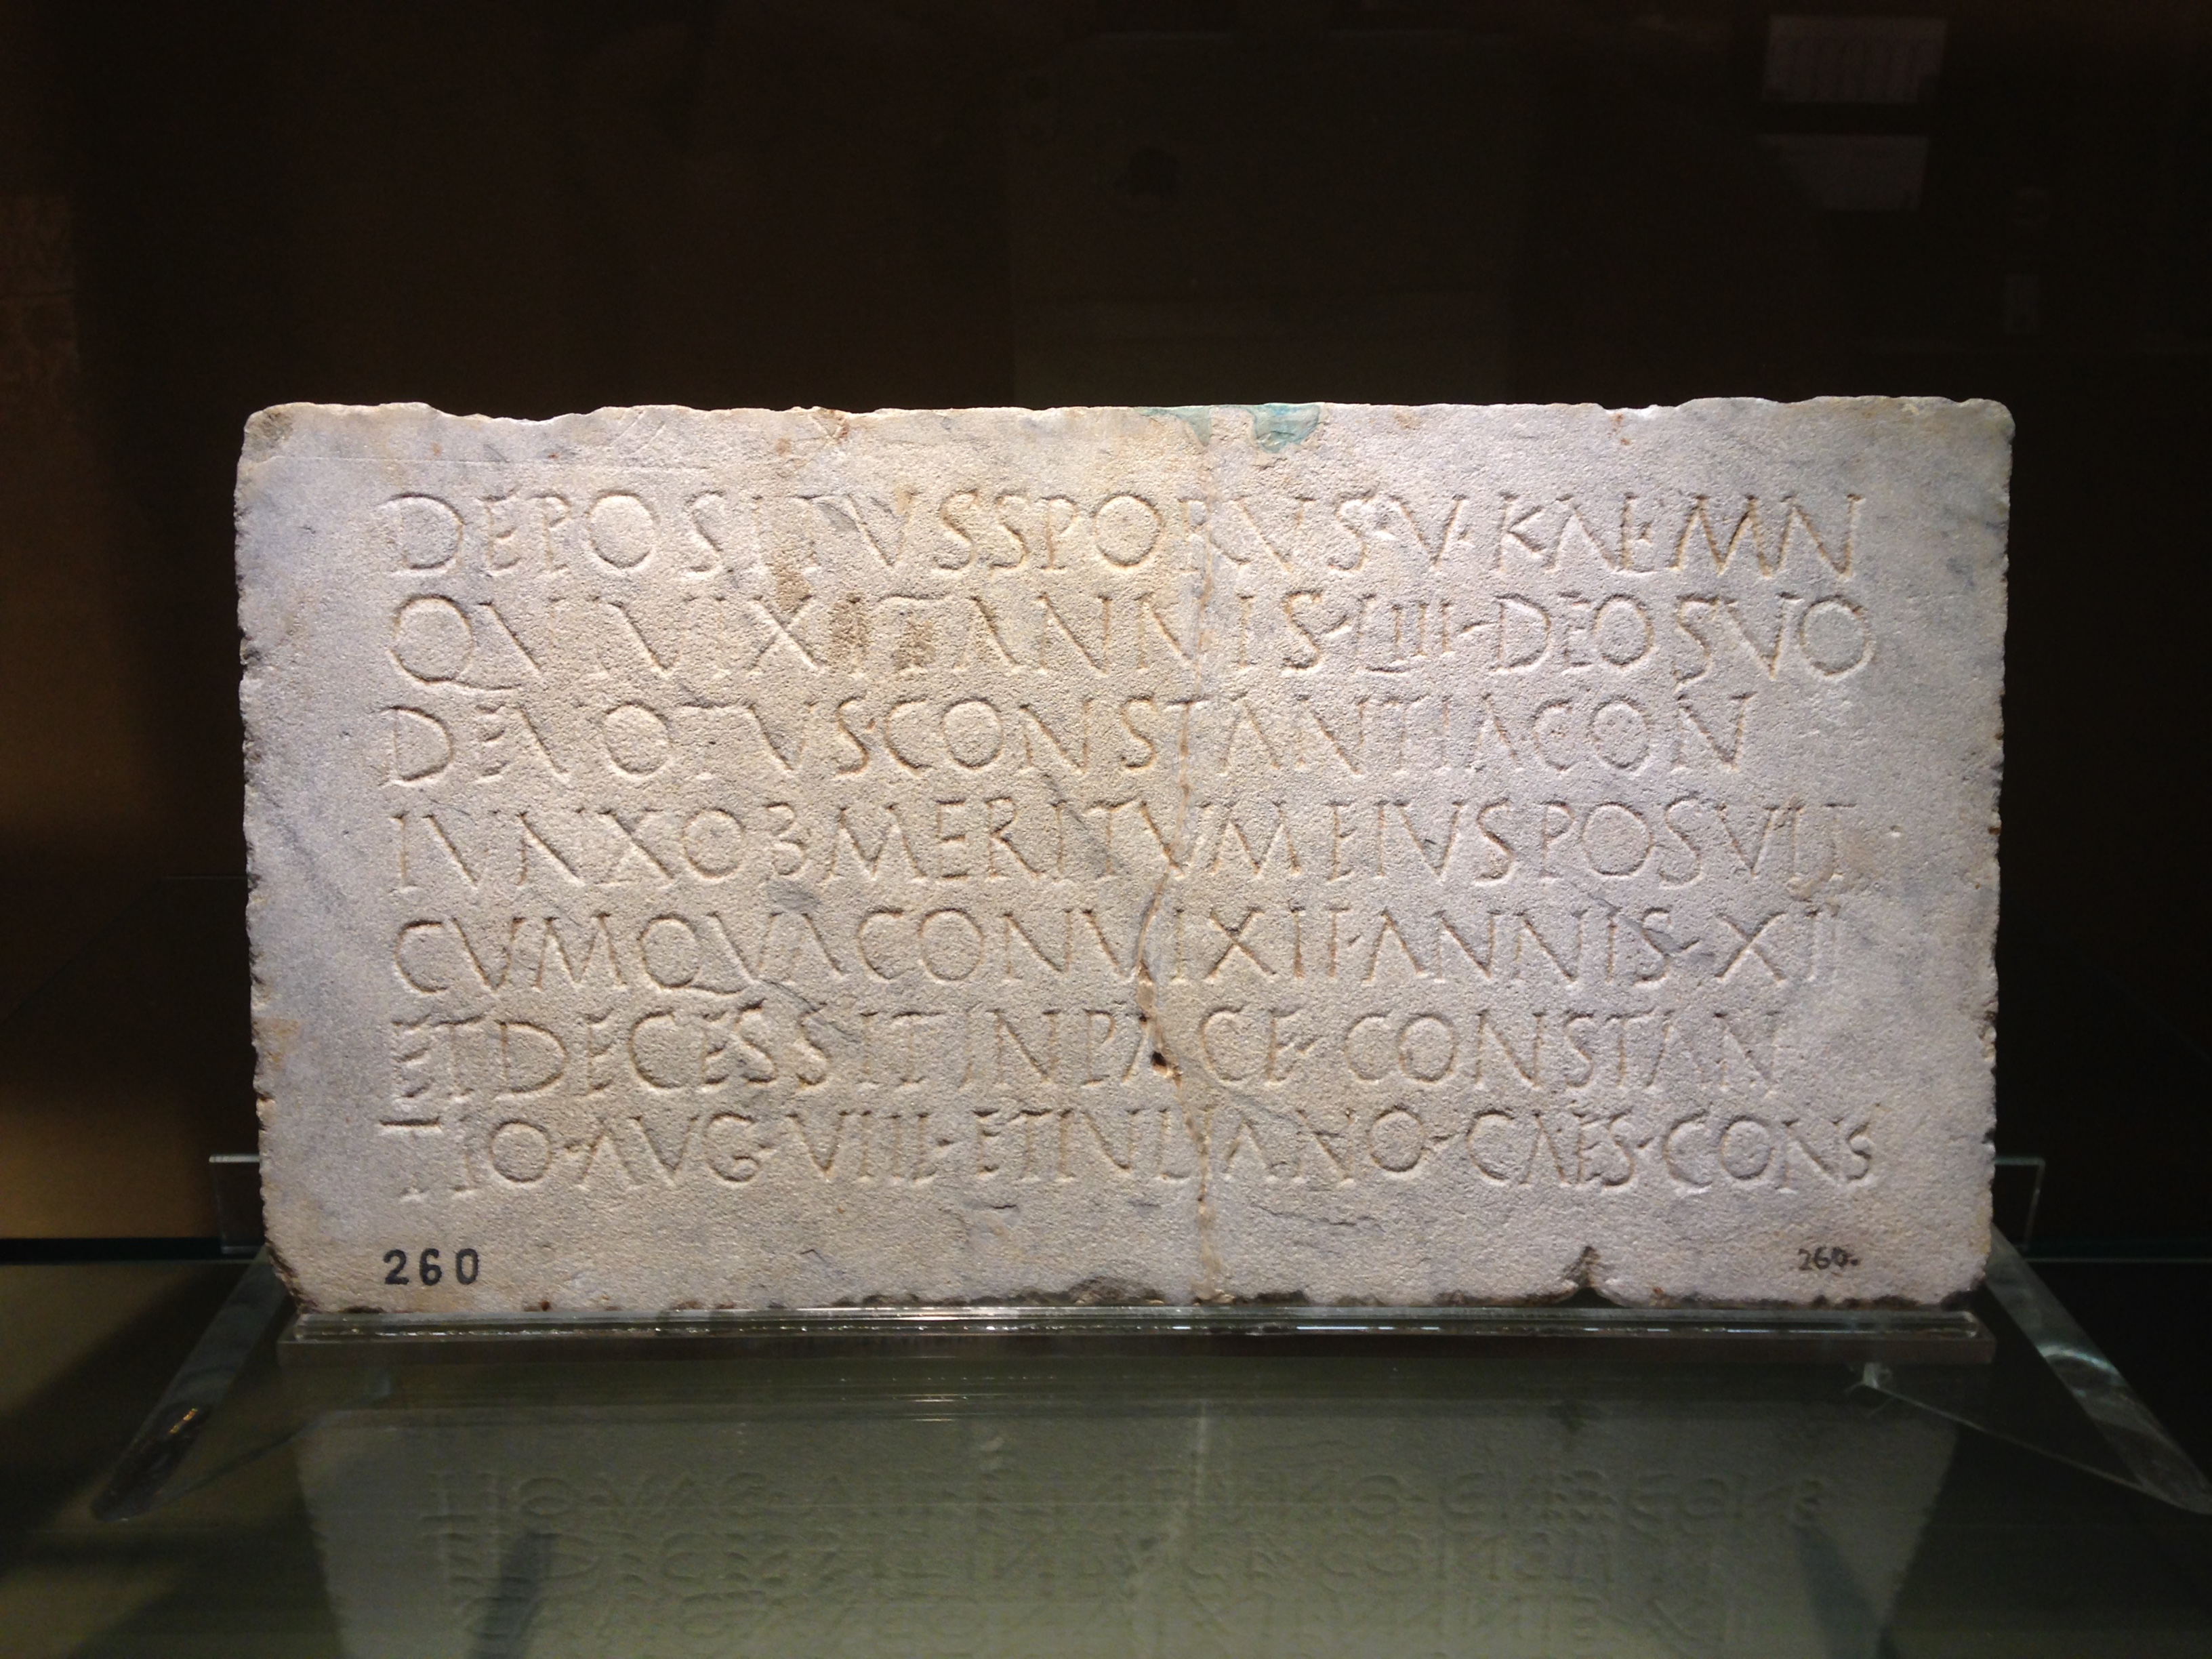
\includegraphics[width=\columnwidth]{Sporus.JPG}
\caption{The Sporus’s inscription}
\label{fig:2}
\end{figure}

The epigraphic research related to San Giovanni catacomb can count on certain informations about the discovery place thanks to Paolo Orsi archeological campaigns. However, looking to previous publications, sometimes it’s necessary a review of the presentations made by Mommsen and Kaibel. In this perspective the main sources of the CIL and IG authors were verified so we had a deeper vision of the relationship between Mommsen and Kaibel and the main sources used, sometimes reevaluating the contribution of this sources. The renovated interest about funerary epigraphy generated new studies about new criteria of dating. The inscriptions dated by the indications of the ``consular couple'' represent an exceptions in the issues about chronological datings (\citealp{FERRUA1947}, nn. 191-208; \citeyear[nn. 191-208]{FERRUA1989}): two were discovered during the excavation conducted by Paolo Orsi (1985) and to them is associated the latin epigraph ``Sporus'' (356) .

The bigger one is entitled to San Giovanni and gave back almost 800 inscriptions, now located for the most part in the Archeological and Regional Museum ‘’Paolo Orsi’’ of Siracusa.; alongside will be placed the 40 headstones recovered in the adjacent hypogea of Villa Landolina, that report compatible datings and formularies.
 
\section{Historical Aspects Of The Catacomb Of S. Giovanni At Syracuse}

\noindent The systematic studies of collective cemeteries in Syracuse started many years ago and, beyond the archaeological surveys, the late antique funerary settlements of Syracuse proposed multiple research cues and paths, as the historical- religious, economic and social nature.
Suburban cemeteries, fanned out from the area of Fusco, in the quarter of Neapolis, to the Santa Lucia area, in the southern part of Acradina, this indicates unequivocally what the perimeter of the city must have already been in the early and mid Roman Empire. The History of the area, which was going to hold the catacombs (San Giovanni, Vigna Cassia and Santa Lucia), spanned the centuries between the classical Greek and late antique ages, gradually giving evidence of quarries (Latomie), water supply systems to the city, characterized by cisterns and aqueducts \citep[682]{COLLINBOUFFIER1987}, handcraft workshops from the beginning of the 4th/3rd century BCE and burials datable to the early and mid Roman Empire. The analysis of the funerary system certifies one hand the dependence on the Roman model, and other the debt in respect of local traditions.

Several interest will be given to structural aspect of the catacomb of S. Giovanni, practice of funeral rituals, ethnic and cultural fruition’s characters, transformation in the use, transformation in the way of using spaces for graves, to complete a general point of view about the phenomena of continuity and innovation as to previous sepulchral arrangements and, in the analysed periods, the facies belonging to the different settling, variegated in the committees’ ideological and religious themes, in choosing monumental types (like the \emph{rotundae}) and decorations, in self-representative aspects, in burial uses. In this perspective we will give particular importance to the study of funerary epigraphy aimed at the writing of ICI Siracusa and the overall interpretation of the monument.

Between 1893 and 1909 the archaeologist Paolo Orsi carried out a series of campaigns in the catacomb of San Giovanni. Detailed reports of those campaigns are recorded at various times in \emph{Notizie degli Scavi}, which constitute an indefeasible starting point. The first incisive studies on Christian subterranean Sicily pertain to Joseph Führer, who dedicates many pages to the catacomb of San Giovanni, whose study is also epigraphic, is based on the previous literature, especially on Paolo Orsi’s discoveries (\citealp[13-39]{FUHRER1897}; \citealp[22-26]{FUHRERSCHULTZE1907}; see also \citealp[276, n. 2]{ORSI1893})
%and \citep[60-61, fig. 5]{SCHULTZE1882} MISSING IN BIBLIOGRAPHY
. In the study of Syracuse cemeteries Orsi \citep[189]{ORSI1900} was the first to see the mixed nature of the burials and their materials (mostly gravestones), openly attesting a kind of pagan-Christian and orthodox-heterodox symbioses %\citep[242-243]{AGNELLO1957a} MISSING IN BIBLIOGRAPHY
. Both Antonio Ferrua and Santi Luigi Agnello within the space of a few years tried to solve the problems relating to the sarcophagus of Adelfia and the more general problem, strictly correlated with the ones just mentioned, of the cemetery genesis and development \citep{FERRUA1952,AGNELLO1956}. It is necessary to record that numerous hypotheses on the genesis and development of the various sectors of the cemetery are ascribable to the account given by inscriptions. Syracuse, thanks to its prolific underground cemeteries, has the larger Christian epigraphic heritage after Rome, kept in the storage of the Soprintendenza di Siracusa.

\section{Topographic And Epigrafic Data To Study The Cemetery}

\noindent Walking across the main gallery, one can retrace the stages of Paolo Orsi’s interventions, being at the entrance of the Catacomb second northern gallery, before the so-called ``tomb of the Saint''. This \emph{arcosolium} is considered a privileged burial on the basis of the following reasons: most of all because of its position, but also because it is a \emph{mensa}type burial closed by a sole slab \citep[292-294]{ORSI1893}. The signs of an ancient rite are easily traceable on the slab, a rite that preceded the coming of Christianity and persisted for centuries up to the present day: the rite of \emph{refrigerium}, which literally means refreshment, cooling \citep{GIUNTELLA1985}. In the Christian ceremony the purpose of a funeral banquet is to benefit the soul of the departed on the anniversary of death, a painful event celebrated as \emph{dies natalis} of the soul to eternal life.

Who was buried in this sepulchre? The question is destined to remain unanswered and only an inscription found nearby could be a clue in this sense. The text says that the owners purchased the sepulchre close to the one of the bishop \emph{Cheperion’s} (\citealp[507-508]{ORSI1895ab}; \citealp[55-58]{RIZZONE2011}), of whom the scanty written sources never make mention. In any case this constructed sarcophagus represent one of the most eminent burials of the catacomb. In the same gallery one cannot ignore the finding of an inscription in many fragments, which is a singular phenomenon of religious contamination.

This inscription, with a Christological monogram at the top, records \emph{Nassiana} ``Christian, who competed with Penelope in moral virtue''. This inscription can only be compared with three examples in the Roman sepulchral \emph{carmina} \citep{CLE}. The circular support of this inscription found close to the ``tomb of the Saint'' has been regarded as a \emph{mensa} (table) for \emph{refrigerium} rite \citep[47]{GIUNTELLA1985}, whose circular form would derive in any case from an evident reuse of a marble disk of classical craftsmanship, with a laurel wreath and berries sculpted on one side \citep[n. 234]{ORSI1895ab}. A wall inscription painted on the extrados of an \emph{arcosolium} in the third northern gallery of the catacomb could be connected with Nassiana’s text. Two lines of the inscription say that ``Sossa outdid (other women) in conjugal love; as for handiworks, without being taught by anyone, Athena herself had taught her how to do marvelous things'' \citep[n. 3]{FERRUA1940}. Both inscriptions unequivocally make use of female figures from the classical world, interpreted as a model also for Christian women either for a deep-rooted usage or making up for the absence of assimilable figures in the Church. This allows one to notice in a 4th century large community cemetery, such as San Giovanni, some phenomena of religious contamination in a period in which Christian epigraphic praxis consolidated itself by then \citep[484]{SGARLATA1999}.

The rotunda derives its name from the deceased Antiochia recorded in the sarcophagus, set inside the ring of tombs, made of blocks and bearing an engraved and rubricated inscription. Whom did this private space belong to? To answer the question, one can rely on a suggestion provided once more by epigraphic testimonies. The gravestones found – on which they put as a rule the deceased’s name, lifespan, date of death and deposition – according to the first excavators’ reports \citep[23-45]{CARINI1873}, attest that the rotunda of Antiochia could have housed women only and this would give credence to the idea that the mausoleum had been used for a female monastic community. The hypothesis needs to be verified, but it is very seductive.

It is evident that the catacomb of San Giovanni was originally a community cemetery, planned for only one type of burial: the \emph{arcosolium} with multiple depositions, which does not require great care for decoration, only transennae. In the topographical and architectural development of the catacomb it appears clear that creating the rotundas breaks up the common burials series, destined to a socially homogeneous Christian community. These changes to the original plan – of the creation of subterranean mausolea both to the north and south of the cemetery – spring from the necessity to create appropriate spaces for the members of the Chruch and above all of the Empire, bringing into question the initial egalitarian choice of the \emph{arcosolium} burials \citep[767]{GRIESHEIMER1989}. In the terminal part of the pious Giovanni’s gallery a monumental sarcophagus, once more hewn out of the rock, can be perceived. Close to the closing wall of the same gallery an inscription was found: it bears the notification of both the consuls of the year 349 %\citep[756, 8]{ORSI1909} MISSING IN BIBLIOGRAPHY
; \citep[89]{AGNELLO1953}. As a rule this date marks the end of the dig works in this sector of the catacomb \citep[75-76]{FERRUA1952}. A arcosolium extrados, in the eastern region, shows traces of a palinsesto, an overlap of paintings and epigraphs than obstruct the identification of the first person buried in this sepulchre, even if recently Vittorio Rizzone proposed the interpretation \emph{Philadelpheia}\footnote{\citet[45-48]{RIZZONE2012}.}. In one of the fossa tombs at the terminal stretch of the main gallery the inscription of Euterpe (IG XIV, 112) has been found, reused to cover the bottom of the tomb, which traditionally marks the end of the dig works of the catacomb (\citealp[75-76]{FERRUA1952}; \citealp[79]{AGNELLO1958}; \citealp[781]{GRIESHEIMER1989}). Beyond the deceased’s biometric data, recorded as ``companion of the Muses'', the epigraph in the last three lines mentions the consuls’ iteration, which allow us to date back to the consulate of the Emperor Constantius, consul for the tenth time, and Julian- Caesar, consul for the third time. So Euterpe died on November 27th 360 A.D. at the age of 22 years and 3 months \citep[524-526]{GUARDUCCI1978}.

In the southern region, more than in other ones, that you can note the transformations that have profoundly undermined its community spirit, which had originally inspired the creation of the catacomb. In the first rotunda of the southern region, is a private space, which was given the name of Marina due to an inscription scratched upon the extrados of the \emph{arcosolium},on the right of the entrance to the short gallery of the bishop Siracosio. The \emph{arcosolium} seems to be enframed by a painted prothyrum, as the still visible column and capital attest, confirming the generalized use of architectural elements in this catacomb, already seen in the rotunda of Antiochia. According to the interpretation of the text, Marina could have been the wife of the patriciuset magister militum Sabinianus, sent by the Emperor Honorius to Spain at the time of barbarian invasions presumably between 409 and 423 \citep[21-22, 40]{FERRUA1989}.

This date would agree with the numerous testimonies given by the inscriptions that have been dated thanks to the notification of the two consuls in office in the year of their death.These testimonies are ascribable to the years of the Emperors Arcadius and Honorius in the first quarter of the 5th century and seem to suggest a link between a few burials of the southern region and the aristocrats’ diaspora from Rome after Alaricus’ advance in 410, who took refuge in Sicily and Africa as they did in other provinces of the Empire \citep[175]{SIRAGO1989}; %\citep[157-158]{VERA1988} MISSING IN BIBLIOGRAPHY
. It is necessary to have a look at the slab of the presumed \emph{arcosolium} of the bishop Siracosio, recorded in one inscription found in an adjacent fossa tomb, which says that the deceased intentionally purchased the sepulchre close to the one of the bishop just mentioned (\emph{IG} XIV, 123: \begin{otherlanguage*}{greek}Ἐνθάδε κῖτε Πολυχ/ρόνιος καὶ Σεραπία. / Ἠγόρασεν τῷτότ/ε καιρῷ / Πολυχρονίου /αἱ Σεραπία ἐπὶ τῷ κυρί/ῳ μου ἐπισκόπῳ Συρα/κοσίῳ\end{otherlanguage*}). It is just a hypothesis seeing in the \emph{arcosolium} with the engraved slab, still in situ, a noble burial for a member of the ecclesiastical hierarchy, for whom, in the absence of other data, according to a letter of pope Gelasius I, an episcopate between 492 and 496 has been proposed (\citealp[223]{NARCISO1952}; \citealp{Carletti:2008aa}). One can clearly distinguish a Christogram with the apocalyptic letters \emph{alpha} and \emph{omega} and two ships in the shape of fish, regarded as making reference to the sacrament of the Eucharist, this is also suggested by the diskettes next to the fishes’ mouths, assimilable to loaves of bread \citep{Sgarlata2013}.

After reading the text of the inscription upon the sarcophagus lid (\emph{CIL} X, 7123: \emph{Ic Adelfia c(larissima) f(emina) / posita conpar / Balericomitis}), one can become aware that it refers only to the woman, not to both husband and wife: here lies \emph{Adelfia, clarissima femina}, wife of the count \emph{Valerius}. Who were therefore \emph{Valerius} and \emph{Adelfia}? The unsolved enigmas of the catacomb of San Giovanni deal with their names and most of all their identification. In reality it is possible to distinguish more than two phases of intervention, which have preceded the creation of the hole for the sarcophagus. At the beginning the internal space of the large niche was scenographically arranged in a terrace pattern with a forceful ascensional effect, not exempt from comparisons \citep[14, plate VII]{NESTORI1973}.The intact Latin inscription of Sporus, dated to 356, which sealed a forma in the main gallery among the ones that join the rotunda of Marina to the one of Adelfia (\citealp[24]{CAVALLARI1872}; \citealp[90]{AGNELLO1953}), would attest that the exploitation of the soil in the area gravitating to the rotunda of Adelfia was already underway after the first half of the 4th century, so confirming the evident anteriority of the six graves cut in the floor to the phase of monumentalization. Both the internal and the external organizations of the large niche (nicchione) would correspond to the first and second phases of intervention respectively, according to the current reconstruction. The problems related to the reconstruction of the third phase seem to be more complicated: the monumentalization phase started with the interment of the sarcophagus and concluded with the acquisition of an aspect comparable to the privileged burials of Roman crypts.

The monument seems to have a less wild internal dynamics of development; the new data (archaeological, historical, epigraphical) \citep[101-108]{SGARLATA1996} allow the scholars to widen the syncopated weave of temporal sequences, to which the analysis of the monument has been pinned by the constant reference to \emph{Valerius Proculus}’ chronology. A new chronology and a different identification of the comes Valerius can be proposed, considering: 1) the evident reuse of the sarcophagus; 2) the topographical development of the catacomb in the area where the sarcophagus has been discovered; 3) the type of monumental intervention, which followed the Roman counterparts, datable to the second half of the 4th century \citep[132-134]{FIOCCHINICOLAI1997}. If Valerius were given a different identity, one could postpone him from the age of Constantine to that of Augustine \citep[15-51]{SGARLATA1998}, on the basis of several accounts about the friendship between the saint from Hippo and a \emph{comes Valerius}, whose physiognomy, is somewhat vague. This friendship, confirmed by the epistles (AUG., Ep. 200, 206, 207; Retr. II, 79 and 88) and the dedication, in 419, of the treatise \emph{De nuptiis et concupiscentia}, is fed on the fight against Pelagianism, which in eastern Sicily had found a fertile soil. The presence of Pelagians in Sicily is attested for certain, according to \emph{Hilarius}’ account under the pontificate of Innocent \citep[429-452]{PIETRI2000} and \emph{Honoreficentia}’s letter, where a \emph{clarissima} based at Syracuse is mentioned. On the island the spread of Pelagian movement looks like a direct consequence of the 410 sacking of Rome and the diaspora of the Roman nobility, of which Pelagius and Celestius were spiritual leaders; the short period they both spent in Sicily was not painless for Christian orthodoxy %\citep[436-437]{PIETRI2001} MISSING IN BIBLIOGRAPHY
 and particularly in Syracuse, as the cemeteries in the area overhanging the Greek theater, intended to serve the communities of the so-called heretics throughout the 5th century \citep{AGNELLO1990}.All the data gathered seems to lead to a different identification of \emph{Valerius} – who, even if he was not Augustine’s correspondent, would be sought in the list of \emph{Valerii} reported in the sources of the first quarter of the 5th century (PLRE II, 1143-44) – and a later chronology of the large niche monumental transformation compared to the one traditionally accepted.

Certainly it is not the case that in this catacomb the traces of the members of ecclesiastical hierarchy are so rare: where are the martyrs? Why is the evidence of bishops, presbyters and deacons so scant? Why is this Christianized elite – to which the will to betray the communal matrix of the original project for a new particularistic conception of funerary space can be attributed – so copious?

To answer the questions will take time, which will assure a greater credibility to what so far seems just a series of suggestions, most of all fed by the re-reading of epigraphic testimonies: the episodic character of the references to burials of bishops, presbyters, deacons and noting that the most significant percentage of evidences pertains to the members of the Church, buried in Syracuse away from their own countries and recorded in wall inscriptions written in Latin – \emph{Auxentius Hispanus episcopus} and \emph{Superianus clerecus de Aquileia} \citep[1 and 6]{FERRUA1940} – as a demonstration that the official language is used by foreigners, who were high clients (the remainder of inscriptions is in Greek), these and many other clues lead to thinking of a less incisive control of the Church in the 5th century than one can commonly believe.

In the rotunda of sarcophagi is surprising the concentration of monumental burials, so that one can think members of the Church commissioned the works here too. What clues are the that could support the hypothesis that the clients belonged to a religious community? To tell the truth, they are scant and among them the epigraph of the blessed virgins Fotina and Filomena deserves to be recorded: the former lived 80 years, the latter 84 (\emph{IG} XIV, 187; \citealp[180]{FERRUA1989}). The sole dated inscription found within this chamber, which is related to the name of Eucarpio, bearing the notification of both the consuls between 339 and 360 \citep[3]{FERRUA1983}, cannot be used for dating; the discovery data, insisting on the fact that the gravestone was found overturned in a \emph{forma} tomb \citep[30-31]{AGNELLO1960}, suggest that the gravestone was reused.

The \emph{cubiculum} of Eusebio has a structure different than other private spaces of the southern region of the catacomb. The name Eusebio derives, once more, from an inscription found on a three level monumental tomb, in the shape of exedra, visible to the left of the \emph{cubiculum} (\emph{IG} XIV, 111). The position and monumentality of the grand \emph{arcosolium}, the formula ``of blessed memory'', the paleographical characters, the identity of pope Eusebius month of death (exiled to Sicily by Maxentius, Eusebius died on 17 August 309 or 310) have suggested to Isidoro Carini that this \emph{arcosolium} could be the pontiff’s temporary sepulchre, whose bones were transferred to Rome and deposited in the catacomb of Callisto. Despite the scholar’s efforts to sustain this theory \citep[134]{CARINI1873}, the physiognomic contours of Eusebius recorded in the inscription remain hazy.

The cubiculum of Eusebio also deserves to be recorded for another testimony, which has a special value for Syracusans: an inscription found in a \emph{forma} tomb, which testifies the worship of Saint Lucy, the patron of Syracuse..No decoration, no distinctive signs characterize the modest burial of Euskia \citep[299-308]{ORSI1895ab}, one of the many graves cut in the soil of the cubiculum \citep[526-528, fig. 164]{GUARDUCCI1978}.

\begin{quotation}
\begin{otherlanguage*}{greek}
\noindent Εὐσκία ἡ ἄμενπτος, ζήσα$<$σα$>$ \\
%Εὐσκία ἡ ἄμενπτος , ζήσα<σα> \\
χρηστῶς καὶ σεμνῶς ἔτη \\
% χρηστῶς καὶ σεμνῶς ἔτη \\ 
πλῖο$<$ν$>$ ἔλαττον κε᾽, ἀνε-\\
% πλῖο<ν>ἔλαττον κε' , ἀνε-\\
παύσετο τῇ ἑορτῇ τῆς κυ-\\ 
% παύσετο τῇ ἑορτῇ τῆς κυ-\\
ρίας μοθ Λουκίας, εἰς ἢν \\
%ρίας μου Λουκίας, εἰς ἢν \\
οὔκ ἐστιν ἐν κώμειον \\
% οὔκ ἐστιν ἐν κώμειον \\
εἰπεῖν, Χρηστειανή, πισ-\\
% εἰπεῖν ,Xρηστειανή , πισ-\\
τή, τέλιος οὖσα, εὐχα-\\ 
% τή ,τέλιοςοὖσα , εὐχα- \\
ριστοῦσα τῷ εἰδίῳ ἀν-\\
% ριστοῦσα τῷ εἰδίῳ ἀν- \\
δρὶ πολλὰς εὐχαρισ-\\
% δρὶ πολλὰς εὐχαρισ-\\
τίασ α \textlatin{\chirho}{} ω εὐομε[ίλητος]
%τίας αⳀω εὐομε[ίλητος].
\end{otherlanguage*}
\end{quotation}

\begin{figure}[hbp]
\centering
 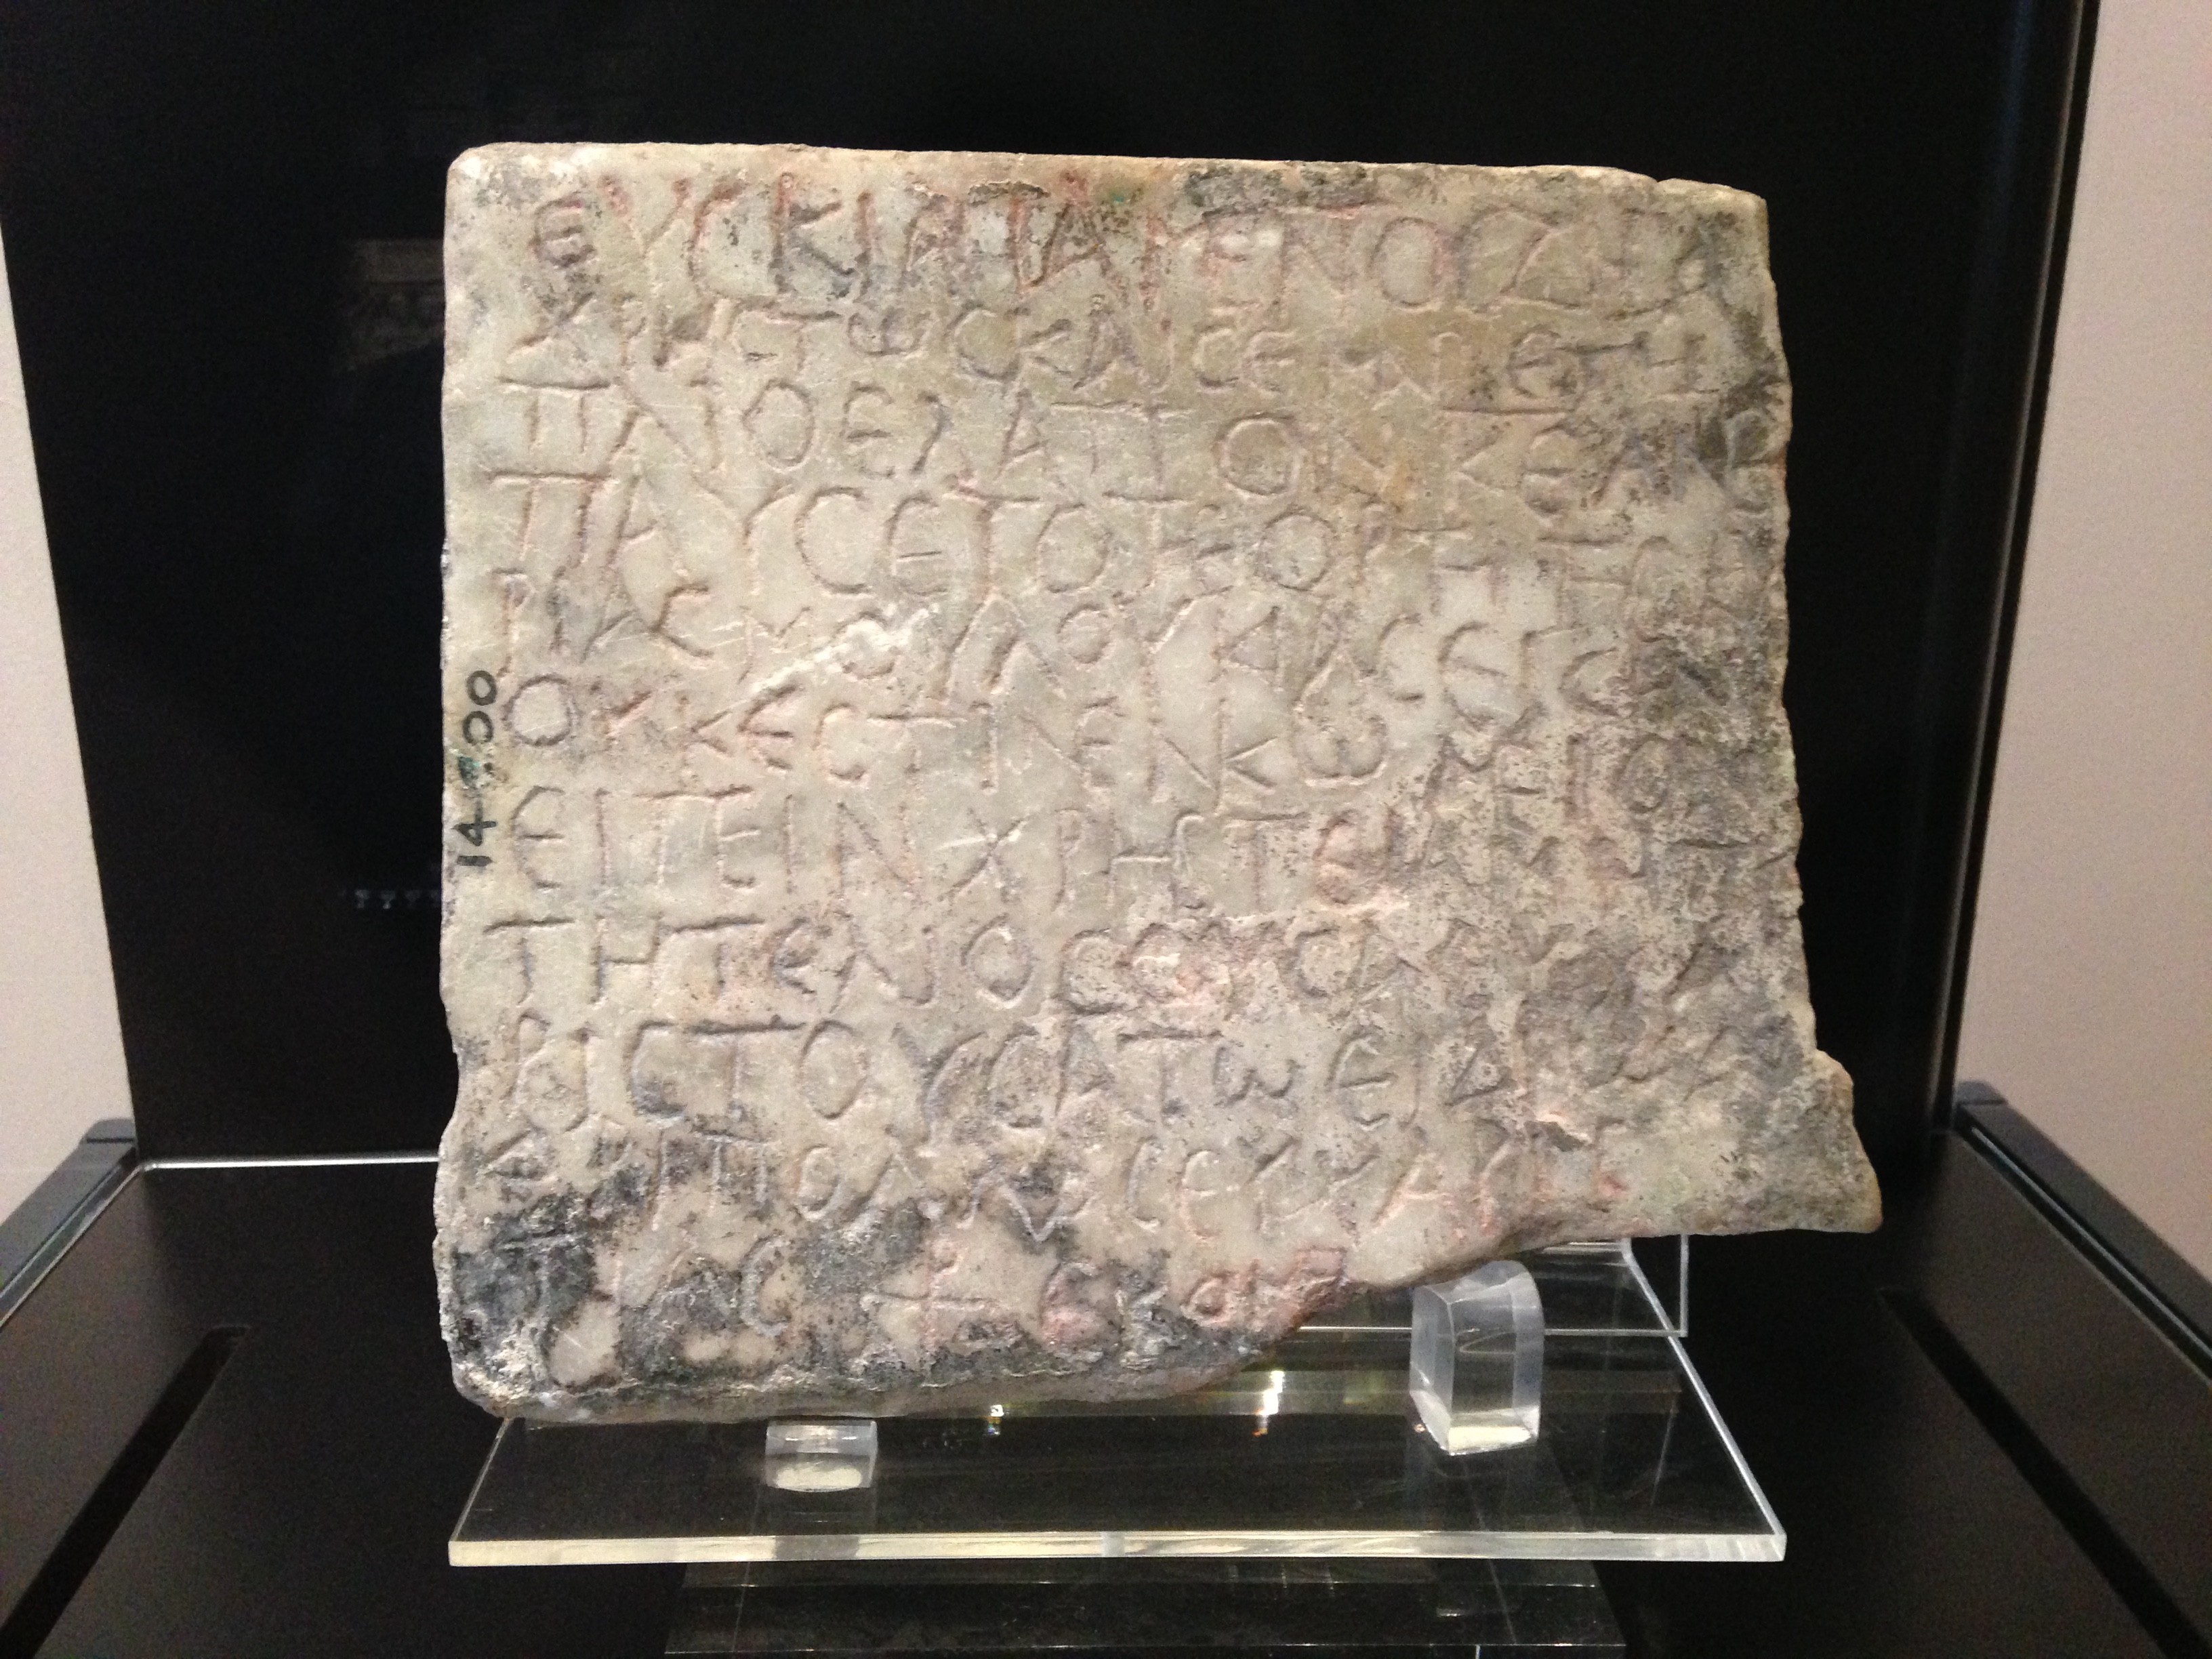
\includegraphics[width=\columnwidth]{Euskia.JPG}
\caption{ The Euskia’s inscription.}
\label{fig:3}
\end{figure}

Euskia, the irreproachable one, who lived her life in good and pure ways for more or less twenty-five years, died on the feast of our lady Lucia, for whom no praise is adequate. She was Christian, faithful (and) perfect, well pleasing to her husband, endued with much grace, affable.

This is the text of the most important Christian epigraph in Syracuse \citep[20]{AGNELLO1953}.The formulae present the typical \emph{elogium}, the retrospective data of the life of the deceased and the Christological monogram flanked by the apocalyptic letters, which are common elements in the inscriptions of the catacombs; it is important since Euskia had been privileged to die on the same day that was sacred to Lucia, patron of Syracusans, a martyr during Diocletian persecutions on the 13th of December 304. The sole doubt of this reconstruction lurks in the term \emph{kyria}, which is referred to Lucia in the epigraph; does one have to interpret it as synonym of \emph{haghia} (saint), which would assure the official character of the worship, or a simple honorary title? Whatever answer one can give, the importance of Euskia’s inscription survives intact, because it testifies if not already the sanctity of Lucia, the local devotion and worship of which the woman was subject in the 5th century in Syracuse.

So this is the first attestation of the cult of Saint Lucia, which confirms the historicity of the Martyrologium Hieronymianum’s account on popular devotion to the Saint, which came through the celebration of a feast from the outset. All of the other evidence refers to successive periods. It is the Greek \emph{martyrion} dated to the end of the 5th century, whose reliability has been debated for a long time and to this day never evidently established \citep[95-135]{MILAZZORIZZONERVO1988}. The inscription, ascribable to the beginning of the 5th century, so would precede the questioned passio and would confirm the antiquity of the cult of Saint Lucia, whose bones were presumably kept in the homonymous catacomb in Syracusee, before George Maniakes, in 1039, transported them to Costantinople. Along with
the inscription of \emph{Iulia Florentina} from Catania \citep[608-610]{RIZZA1964}, the epigraph of Euskia is the most ancient Sicilian document that one could relate to the experience of martyrdom.

\section{Epigraphic Population: Formularies And Identity-Making Characteristics}

The 800 inscriptions found in the San Giovanni catacomb give us an idea about the epigraphic approach and the society of that time. One single epigraph can mention more than one person so the number of remembered deceased is superior than the number of inscriptions; starting from this number it’s possible to launch a demographic investigation to determine the expectation of life.

In Syracuse all the social classes were affected with inexorable mortality; high percentage among young people (under 20) and extremely low percentage among old people (over 60). The demographic data follow standard hypothesis: male mortality between 15 and 34 years and female mortality between 20 and 24 years (reproductive period). The life expectancy for both genders was around 29 years.

\begin{figure}[hbp]
\centering
 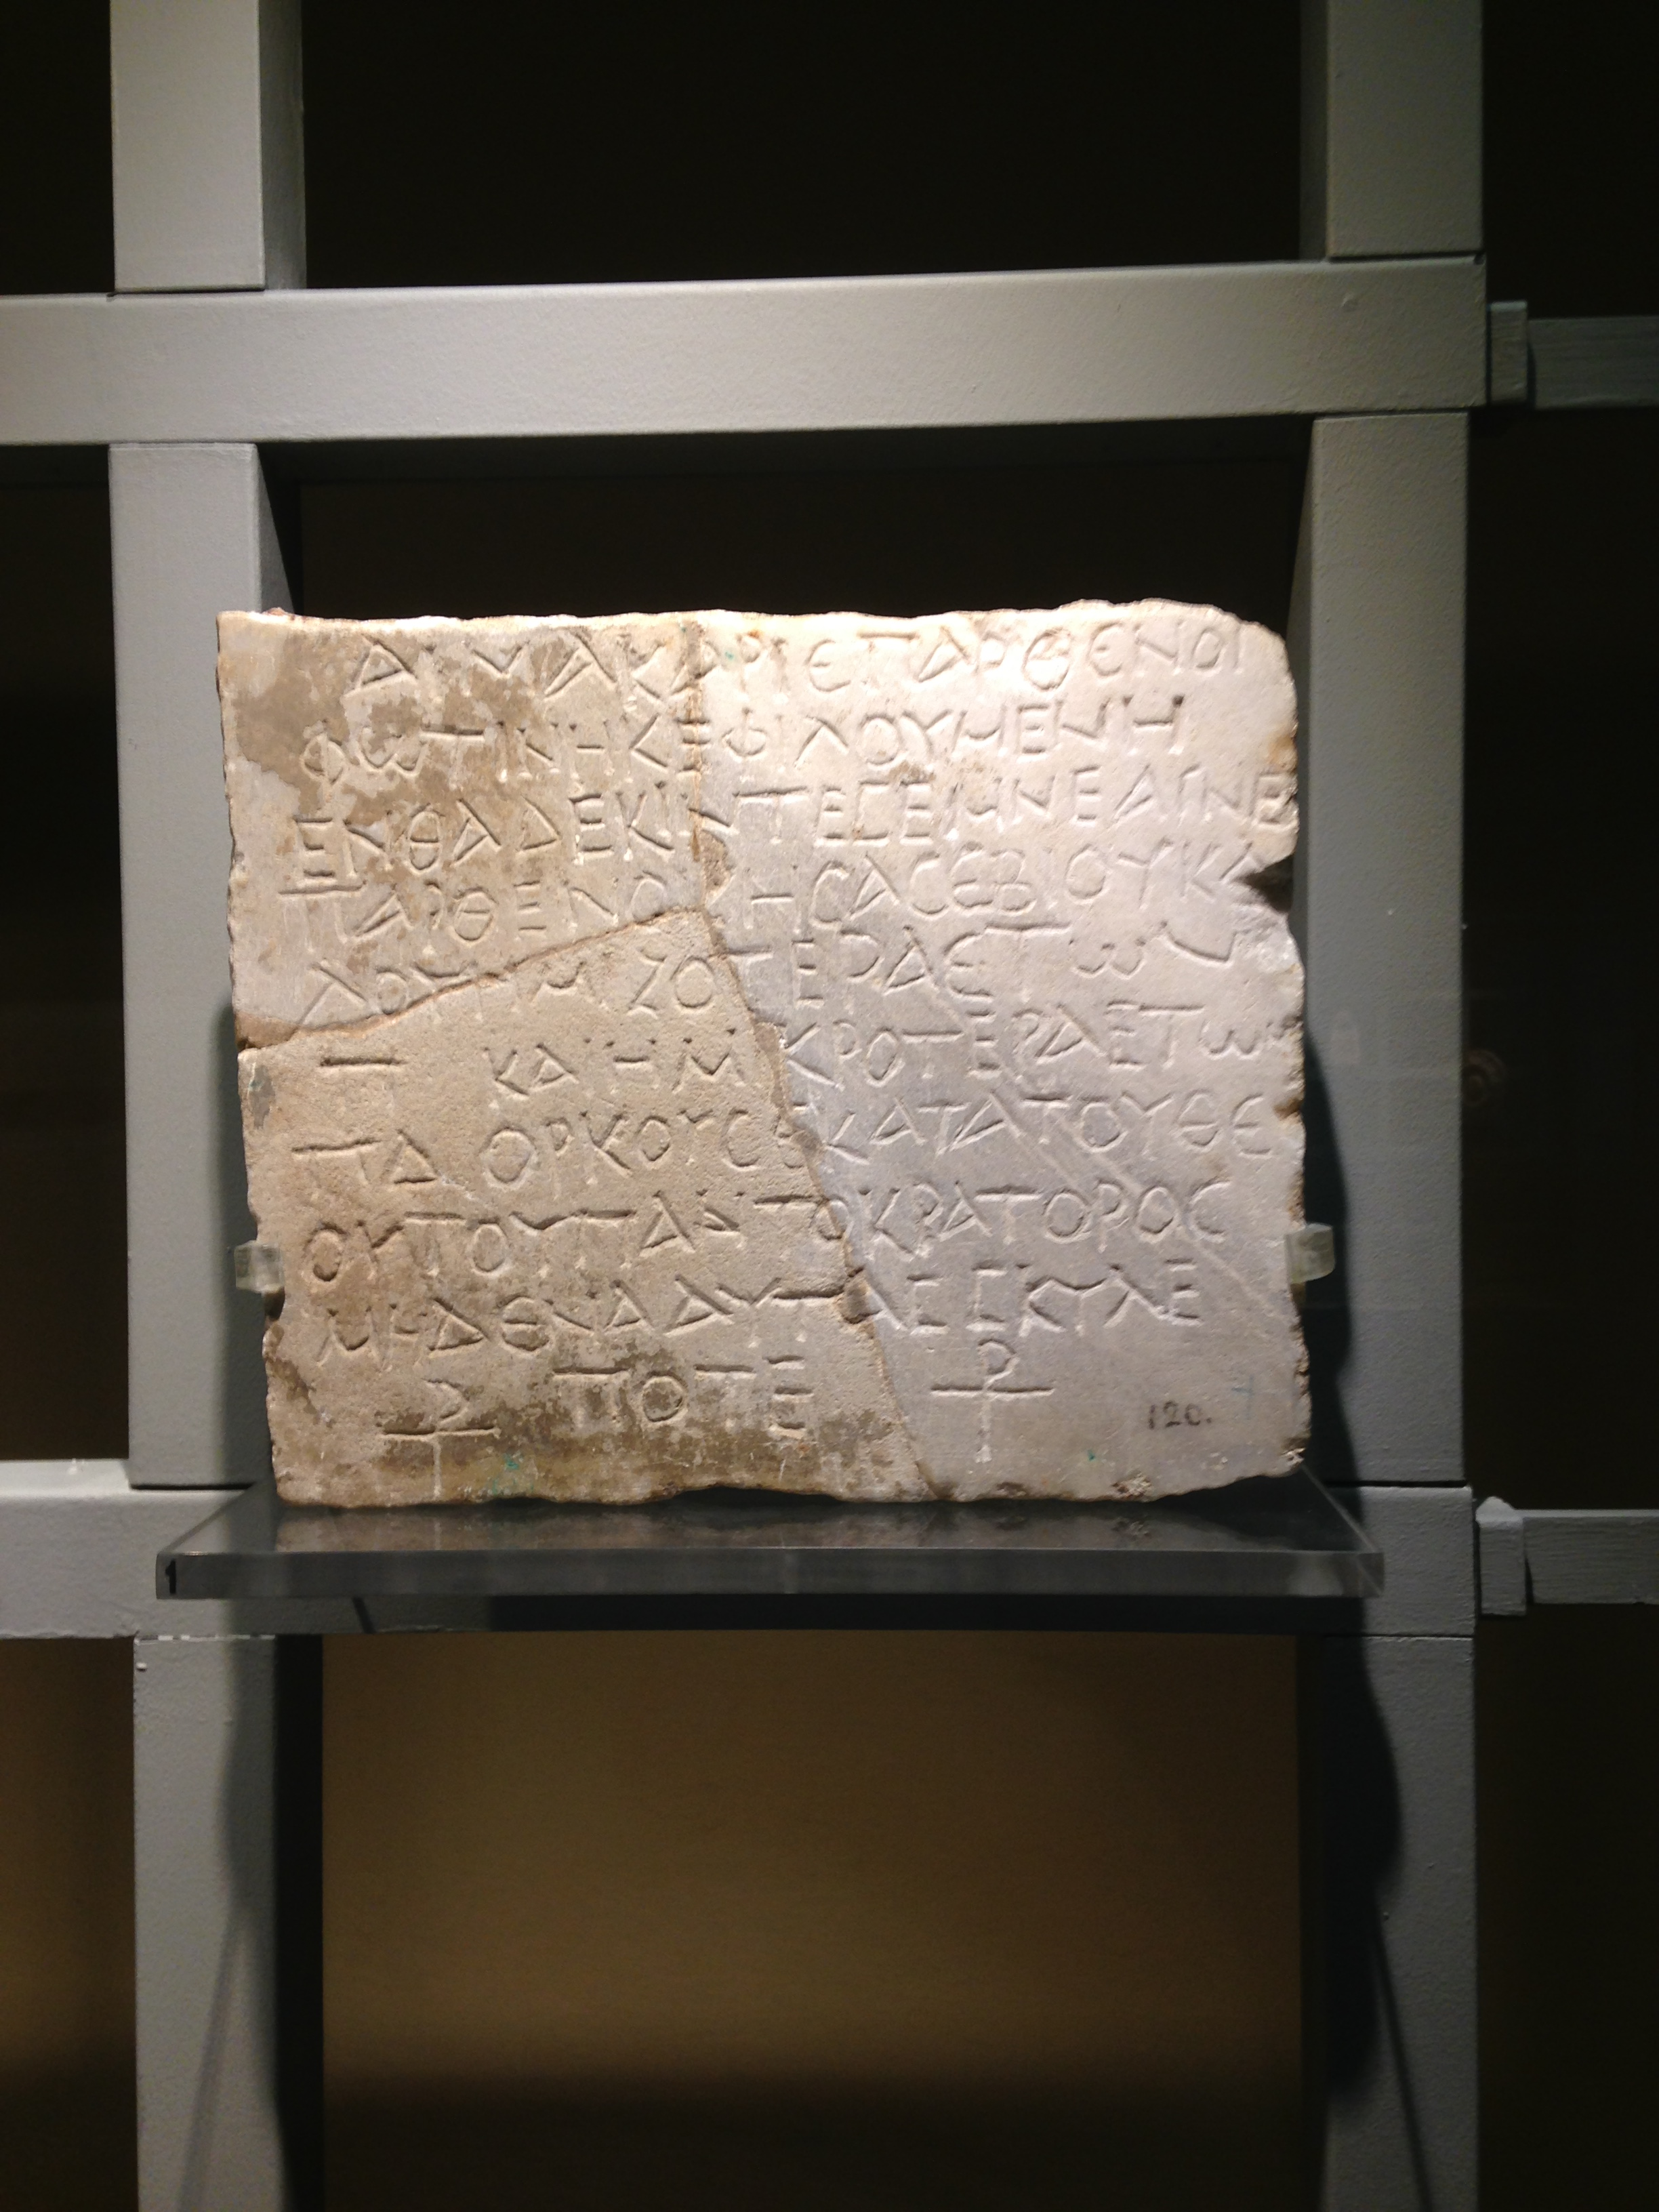
\includegraphics[width=\columnwidth]{FotinaeFilomena.JPG}
\caption{The Fotina and Filomena’s inscription.}
\label{fig:4}
\end{figure}


We focus on the decesead elogistic formulary that help to increase the study about social aspects. In our research there are few examples of nuptial terminology, all referred to female deceased: \emph{compar, coniunx}, 
\begin{otherlanguage*}{greek}σύμβιος, νυμφη\end{otherlanguage*}
.\footnote{V. cat. n. XX-XXI} It marks a common characteristic: the priority in honoring the wives more than the husbands. Linked to this is the importance given to the sexual integrity of the dead person, in fact the concept of virginity in the nuptial context is particularly marked trhough the adjective virginius-a o \begin{otherlanguage*}{greek}παρθενικός-ή.\end{otherlanguage*}
\footnote{See also \citet[129-130]{SGARLATA1991} \citet[493]{CARINI1887}; CIL X, 7168, 2-4; \citet[5, 22, 44]{ORSI1893}; \citet[6, 7]{FUHRER1897}; \citep[21/29, 38, 39, 43, 45, 48, 58, 60, 69]{FERRUA1983}; IGCVO 127, 655, 778, 946,950, 1036, 1069 e 1366. Cat. n. XX \citep[214]{ORSI1896}. See. cat. n. XX-XXI} The word \begin{otherlanguage*}{greek}παρθένος\end{otherlanguage*} 
appears seven times and always referred to women. Women who chose monastic life leave behind them all the duties of nuptial life so probably the had a much longer life expectancy than married women. One impressive example is the one of ``Fotina e Filomena'', consecrate virgins (80 and 84 years old, as stated above). Such a long lifespan, for the centuries under examination, finds a justification only in considering that both the women chose a monastic-type life, avoiding the slow attrition due to diverse factors: precocious age weddings, consecutive childbirths since their early adolescence, abortive practices by makeshift means and, lastly, even after the dangerous age of 25/30, the overwork that household management and hygienic-sanitary conditions involve. The biometric data recorded in the inscriptions confirmed in Syracusan sample as well \citep{SGARLATA1991}, testify that life expectancy at birth, considering the high rates of infant mortality, was not over 30 years on average, both for men and women; this datum is not surprising, if one bears in mind that the average span life was about 45 years still in the first half of the nineteenth century.



\section{Conclusions}

The new approach to the catacomb of San Giovanni brings many things into question, such as the fideistic attitude of those, who have studied this monument and have looked at the epigraphic evidence for chronological purpose. Rereading Orsi’s excavations data unequivocally shows how itinerant are the dated inscriptions within the cemetery – with the exception of three, whose discovery data attest their permanence in the original position (\citealp[43-50, 352-353]{ORSI1896}; \citealp[90, 97]{AGNELLO1953}) – which advises the scholars against using them to seal chronologically the diverse sectors. It would be profitable to draw a map of reuse, which is certainly the most striking phenomenon detected thus far in Orsi’s accounts, more than continuing to date the works in the galleries on the basis of dated inscriptions found in their terminal part. But, even underestimating this phenomenon, the inscriptions datable to the years around 350 and the ones, more considerable numerically, that bear the notifications of both the consuls between the end of the 4th century and the first half of the 5th century, have been seen both in the northern region and the southern one, as well as the main gallery \citep[109, n. 62]{SGARLATA1996}, which excludes drawing conclusions on the internal development of the catacomb. A datum, however, is worth considering: epigraphic evidence and intense exploitation of funerary space attest the vitality of the area that gravitates around the three southern rotundas after the end of the great works of excavations. What appears episodic in the other sectors of the catacomb – for example the so- called sepulchre of the Saint – becomes constant in the southern region, where diverse types of intervention on pre- existent structures and high percentage of dated inscriptions demonstrate, still in the first half of the 5th century, a special concentration of interest. During the work on the editing of ICI, the first certain fact we acquire studying the inscriptions is that the dated ones are almost always reemployed and itinerant within the catacomb, with the exceptions just mentioned. We have to make also another consideration that will allow us, once ended the work of cataloguing and copying the epigraphs, to deal with the language question in a deeper and more articulated way. Also the linguistic choice recorded in epigraphic evidence is worth considering: the inscriptions in Greek surpass by far, with a rate of about 90\%, the ones in Latin. About motivations of language choice not all the researchers agree, discerning between the language example provided by the christian graveyards inscriptions and the one expressed by the whole citizenry. It is worth to mention what Kalle Korhonen affirms: ``moreover, it must be painted out that even if 90\% of ca. 1.100 inscriptions from the catacombs of Syracuse are in Greek, we are not allowed to conclude that 90\% of the population of Syracuse was Greek from the 3rd to the 5th. It is likely that the non-Christian parts of the population, which was notable until the 4th century, were not buried in catacombs and their epithaphs have mostly perished'' \citep[124- 125]{KORHONEN2011}.

Assuming this, one could state that in Sicily religious conversion is not a linguistic conversion, proving wrong the theory according to which in urban centers Christianization would bring along an early diffusion of Latin, whereas the pagus, keeping the use of Greek, would keep its distance from Christianity, at least until the early 5th century, during which signs of both linguistic and religious conversion would become a little more evident \citep[545]{manganaro_greco_1993}. Epigraphic documentation records, for Syracuse and its territory, as for Catania, a marked preponderance of the use of Greek still in the 5th century; so in urban centers Christianization does not bring an early diffusion of Latin, which was prerogative of high and foreign clients, as only the use of Greek in the \emph{pagus} does not prove the extraneousness to the process of diffusion of the new creed still at the beginning of the 5th century. The idea according
to which ``several signs of religious dissidence, in the 5th and 6th centuries, can be recognized only in peripheral rural areas, where the level of ecclesiastical control was slack. In these centuries conventional superstitions were slowly relegated to periphery'' \citep{CRACCORUGGINI1998} needs to be dampened.

The cemetery of San Giovanni has subtly given back, even if in a more hidden way, several testimonies of ideological commixture, which do not distinguish it from other communal cemeteries in Syracuse, where phenomena of ``religious dissidence'' are more readable \citep{SGARLATA2003}. The catacomb was created in different cultural and religious contexts (after the Peace of the Church). The cemeteries distribution (both of private and community law) and topography of funerary monuments in the suburban area of Acradina, between the 3rd and 5th centuries, reflect well a diversified situation within a few hundred meters radius. To understand that, one needs to take account of the relationship between paganism and Christianity, orthodoxy and heterodoxy (most of all for the 5th century) \citep{MACMULLEN1997}, which is not only a Sicilian problem, even if it is strongly sensed in the island \citep[59]{GRECO1999}.

\nocite{Orsi:1896aa}

\bibliographystyle{sapauth-eng}
\bibliography{../../EAGLE}

\end{document}


